\documentclass[11pt,a5paper]{article}

\usepackage[T1]{fontenc}
\usepackage[utf8]{inputenc}
\usepackage{lmodern, microtype}
\usepackage[estonian]{babel}
%\usepackage[per=fraction, expproduct=cdot, decimalsymbol=comma, inter-unit-product=\cdot]{siunitx}
\usepackage{siunitx}
\sisetup{inter-unit-product=\ensuremath{{}\cdot{}}, per-mode=fraction, exponent-product=\cdot, output-decimal-marker={,}}
\usepackage{graphicx}
\usepackage{wrapfig}
\usepackage{subfig}
\usepackage{tikz}
\usetikzlibrary{arrows.meta}
\usepackage[european]{circuitikz}
\tikzset{component/.style={draw,thick,circle,fill=white,minimum size=0.75cm,inner sep=0pt}}
\usepackage{amsmath,amssymb}
\usepackage{amsfonts}
\usepackage{physics}
\usepackage[hidelinks]{hyperref}
\usepackage{csquotes}
\usepackage{caption}
\usepackage{enumitem}
\topmargin=-3.0cm \textheight=19cm \textwidth=12.9cm
\oddsidemargin=-1.5cm  \evensidemargin=-1.5cm
\setlength{\parindent}{0pt} \setlength{\parskip}{6pt} \sloppy
\sloppy \relpenalty=10000 \binoppenalty=10000
\pagestyle{empty}

\newcommand{\numb}[1]{\vspace{5pt}\textbf{\large #1}}
\newcommand{\nimi}[1]{(\textsl{\small #1})}
\newcommand{\punktid}[1]{(\emph{#1~p.})}
\newcounter{ylesanne}
\newcommand{\yl}[1]{\addtocounter{ylesanne}{1}\numb{\theylesanne.} \nimi{#1} \newblock{}}
%\newcommand{\autor}[1]{}% Kasuta võistluse ajal
\newcommand{\autor}[1]{\emph{ Autor: #1}}% Kasuta kui vaja autorit

\begin{document}
\begin{center}
  \textbf{\Large Eesti koolinoorte 35.\ füüsika lahtine võistlus} \par
  \emph{30.\ november 2024. a.\\Vanema rühma lahendused (11.--12.\ klass)}
\end{center}

\DeclareSIUnit\aasta{aasta}

\yl{VABASUKELDUMINE}
\punktid{6} \autor{Jarl Patrick Paide}

Sukelduja vabalangemine hakkab pihta siis, kui üleslükkejõud muutub väiksemaks kui raskusjõud. Selleks peab sukelduja ruumala olema $V_1 = \frac{m_0}{\rho} = \SI{75}{l}$. Selle saavutamiseks peab sukelduja kopsu ruumal olema $V_{k2} = V_{k} - (V_0 - V_1) = \SI{3}{l}$. Meil on sukeldumise ajal isotermiline protsess, seega kops saavutab vajaliku ruumala rõhu $P_1 = \frac{P_0V_{k}}{V_{k2}} = \SI{405200}{Pa}$ juures. Selline rõhk saavutatakse sügavusel $H = \frac{P_1 - P_0}{\rho g} = \SI{31}{m}$

\yl{KAKS KERA}
\punktid{6} \autor{Jarl Patrick Paide}

Olgu kera tihedus $\rho$, raadius $R$ ja seega mass $M = \frac{4}{3}\pi R^3 \rho$. Kahe keha vaheline gravitatsioonijõud on $F = \frac{G M^2}{4R^2}$. Et kerad saaksid olla ringorbiidil nurkkiirusel $\omega$, on vaja neile rakendada tsentripetaaljõudu $F = M \omega^2 R$. Pannes vastavad jõud võrduma, saame $\frac{G M}{4 R^3} = \omega^2$ ja asendades sinna $M$ sisse, saame, et tihedus $\rho = \frac{3\omega^2}{\pi G}$.

\yl{VALGUSKAABEL}
\punktid{8} \autor{Richard Luhtaru}

Defineerime nurgad $\alpha$ ja $\beta$ nagu joonisel. Valgus levib ilma kadudeta siis, kui $\beta$ on piisavalt suur ja kaabli südamikus toimub täielik sisepeegeldumine. Seega piirjuhul
\begin{equation*}
    n_1 \sin \beta = n_2.
\end{equation*}

\begin{figure}[h]
    \centering
    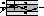
\includegraphics[width=.7\linewidth]{valguskaabel_lah_joonis.pdf}
\end{figure}

Murdumisseadusest saame samuti
\begin{equation*}
    n_0 \sin \theta_0 = n_1 \sin \alpha \implies n_0 \text{NA} = n_1 \sin \alpha \implies \text{NA} = \frac{n_1 \sin \alpha}{n_0}.
\end{equation*}

Kuna $\alpha$ ja $\beta$ on täisnurkse kolmnurga nurgad, siis $\beta = \ang{90} - \alpha$, seega $\sin \beta = \cos \alpha$. Seega
\begin{equation*}
    n_1 \cos\alpha = n_2 \implies \cos \alpha = \frac{n_2}{n_1} \implies \sin\alpha = \sqrt{1-\cos^2\alpha} = \sqrt{1-\left(\frac{n_2}{n_1}\right)^2}
\end{equation*}
ning
\begin{equation*}
    \text{NA} = \frac{n_1}{n_0}\sin\alpha = \frac{n_1}{n_0}\sqrt{1-\left(\frac{n_2}{n_1}\right)^2} = \frac{\sqrt{n_1^2-n_2^2}}{n_0}.
\end{equation*}



\yl{RONGIÜHENDUS}
\punktid{10} \autor{Jonatan Kalmus}

Olgu rongide kiirus $v$ ning $T$ rongide vaheline aeg, s.t. iga ajavahemiku $T$ järel siseneb raudteelõiku üks rong. (Kuna kiirus on ühtlane, väljub ka iga ajavahemiku $T$ järel üks rong, aga mitte tingimata samal ajahetkel.) Maksimaalne raudteelõigu läbilaskmisvõime vastab seega minimaalsele rongide vahelisele ajale $T$. Selle aja jooksul peab rong läbima iseenda pikkuse $l$ ning rongidevahelise ohutu vahemaa ehk kahekordse pidurdusmaa:
\begin{equation*}
    2s = 2\frac{v^2-0^2}{2a}=\frac{v^2}{a},
\end{equation*}
Saame seega võrrandi 
\begin{equation*}
    T = \frac{2s+l}{v} = \frac{\frac{v^2}{a}+l}{v} = \frac{v}{a} + \frac{l}{v} \tag{I}
\end{equation*}

Kasutades vihjet saame
\begin{align*}
    T &= \underbrace{\frac{v}{a}}_{x} + \underbrace{\frac{l}{v}}_{y} \geq 2 \sqrt{\underbrace{\frac{v}{a}}_{x} \cdot \underbrace{\frac{l}{v}}_{y}} 
    = 2\sqrt{\frac{l}{a}} = 2 \sqrt{\frac{\SI{900}{m}}{\SI{1}{m/s^2}}} = \SI{60}{s} \tag{II}
\end{align*}

Korrutades võrrandi $\text{(I)}$ kiirusega $v$ saame ruutvõrrandi optimaalse kiiruse leidmiseks:
\begin{align*}
    Tv = \frac{v^2}{a}+l \qquad &\Longleftrightarrow \qquad v^2 - Tav + l = 0 \\
                                &\Longleftrightarrow \qquad v = \frac{Ta \pm \sqrt{(Ta)^2 - 4l}}{2} \\
                                &\Longleftrightarrow \qquad v = \frac{60 \pm \sqrt{60^2 - 4\cdot 900}}{2} = \SI{30}{(m/s)}
\end{align*}

Ülesande võib lahendada ka tuletisega. Sel juhul leiame otse minimaalsele ajale vastava kiiruse:
$$
T'(v) = \frac{1}{a}-\frac{l}{v^2} = 0 \qquad \Longrightarrow \qquad v = \sqrt{\frac{l}{a}} = \sqrt{\frac{\SI{900}{m}}{\SI{1}{m/s^2}}} = \SI{30}{(m/s)}
$$



\yl{VÄRSKE ÕHK}
\punktid{10} \autor{Jaan Kalda}

Toas olijad toodavad süsihappegaasi $3v=\SI{51}{\litre\per\hour}$ ja see on kõik vaja läbi õhuakna välja lasta. Vahetugu tunnis õhu ruumala $V$; sellisel juhul tuleb sisse süsihappegaasi ruumalaga $V\cdot \frac{0.42}{1000}$ (peale toas soojenemist ja paisumist) ja välja läheb ruumalaga $V\cdot \frac{1}{1000}$. Seega $3v=V\cdot \frac{1-0.42}{1000}$, millest $V=3v\cdot \frac{1000}{0.58}=\SI{88}{\m\cubed}$. Sellele ruumalale vastab moolide arv $n=\frac{pV}{RT_1}$, mille soojendamiseks kulub energiat $Q=nC_P(T_1-T_0)=pV \frac{C_P}R(1-\frac{T_0}{T_1})$, kus õhu molaarne  erisoojus konstantsel rõhul $C_P=\frac 72R$ ja $T_i=t_i+\SI{273}{\kelvin}$.
Siit saame $Q=\SI{3150}{\kilo\J}$, mis annab võimsuseks $P=Q/\SI{3600}{\s}=\SI{876}\watt$.



\yl{VARI}
\punktid{10} \autor{Jaan Kalda}

\begin{figure}[h]
    \centering
    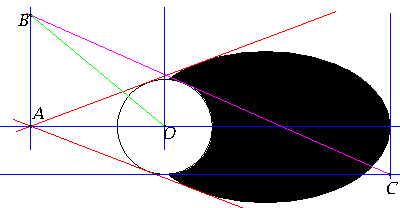
\includegraphics[width=.7\linewidth]{vari-lah.pdf}
\end{figure}

Lambi projektsiooni lauapinnale leiame kui ülaltvaates kera ja varju puutujate lõikepunkti $A$ (vt joonist). Tõmbame nüüd ringil horisontaalse puutuja ja vaatleme seda kui lauapinna vertikaallõike joont. Tõmbame varjule vertikaalpuutuja, selle lõikepunkt $C$ vasttõmmatud horisontaaljoonega on varju kaugeima punkti asukoht vaadeldaval vertikaallõikel. Tõmbame punktist $C$ puutuja ringjoonele ja punktist $A$ vertikaaljoone; nende lõikepunkt $B$ on lambi asukoht vertikaallõikel. Lambi kaugus vastab lõigule $OB$, joonlauaga mõõtes leiame, et see on umbes \SI{3.7}{} korda suurem, kui kera raadius.



\newpage
\yl{ÄIKESETORM}
\punktid{10} \autor{Jarl Patrick Paide}

Võime eeldada, et äike käitub löögi hetkel juhtmena, mis on sirge ja maaga risti, voolutugevusega $I = \SI{30000}{A}$. Leiame äikese kauguse $r = t\cdot v_{õ} = \SI{3400}{m}$. Seega äikese poolt tekitatud magnetvälja muutus on $\Delta B = \frac{\mu I}{2\pi r} = \SI{1.765}{\micro T}$. Kuna äike lööb maapinnaga risti, siis on äikese poolt tekitatud magnetväli horisontaalne maapinnaga. Maa magnetvälja horisontaalne komponent (mis näitab põhja suunda) on $B_{hor} = \sin{\alpha}B = \SI{14.62}{\micro T}$. Põhja suund on maksimaalselt mõjutatud siis, kui Maa magnetvälja horisontaalne komponent on risti äikese poolt tekitatud magnetvälja muuduga. Seega muutus on $\beta = \arcsin{\frac{\Delta B}{B_{hor}}} = 6.9^{\circ}$



\yl{KÄRU}
\punktid{12} \autor{Jaan Kalda}

Lahendame ülesande virtuaalse nihke meetodil: oletame, et piirjuhul, kui käru on libisemise piiril ja liigub aeglaselt allapoole vahemaa $x$ võrra. Alustuseks paneme tähele, et vähemalt ühed rattad peavad libisema. Kui libiseksid tagumised rattad, siis mõjuks jõuülekanne tagumiste rataste telje suhtes jõumomendiga $T=F_hR$, kus $F_h=\mu N$ on hõõrdejõud ja $R$ - ratta raadius, see tuleneb jõumomentide tasakaalutingimusest telje suhtes. Energia jäävusest johtuvalt kannab jõuülekanne selle momendi esimestele ratastele $\frac 98$ korda suuremana, mistõttu peaks esimestele ratastele mõjuma hõõrdejõud $\frac 98\mu N$, mis ei ole aga võimalik, sest maksimaalne hõõrdejõud on $\mu N$. Seega tagumised rattad ei saa libiseda ja seda peavad tegema esimesed. Kui käru liigub alla vahemaa $x$ võrra, siis  tagumised rattad pöörduvad nurga $\phi_t=x/R$ võrra ning esimesed rattad --- nurga $\frac 89x/R$ võrra. Seega libisevad esimesed rattad vahemaa $s=x-\frac 89x=\frac x9$ võrra, mille käigus dissipeerub hõõrdejõu töö tulemusel soojushulk $\mu N\frac x9$. Energia jäävuse tõttu peab see olema võrdne vankri potentsiaalse energia vähenemisega, $\mu N\frac x9=mgx\sin\alpha$, kus $mg=2N/\cos\alpha$ on vankri mass. Seega $\tan\alpha = \frac \mu{18}$.




\yl{KONDENSAATORID}
\punktid{12} \autor{Uku Andreas Reigo}

Kondensaatori mahtuvusest $C = \frac{\varepsilon_0 b^2}{d}$ järeldub, et meil $C_1 = \frac{\varepsilon_0 b^2}{d}$ ja $C_2 = 4C_1$.
Jadamisi ühendatud kondensaatorite jaoks on $C_{tot} = \frac{1}{\frac{1}{C_1} + \frac{1}{4C_1}} = \frac{4C_1}{5}$, seega laeng kõigil plaatidel on $Q = CU = \frac{4UC_1}{5}$. Pinge esimesel kondensaatoril on $U_1 = \frac{Q}{C_1} = \frac{4U}{5}$ ning teisel kondensaatoril järelikult $U_2 = \frac{U}{5}$. Vastavalt, kuivõrd elektriväli kondensaatoris on $E=\frac{U}{d}$, rakendub osakesele esimese kondensaatori alas kiirendus $a_1 = \frac{U_1q}{dm} = \frac{4Uq}{5dm}$ ning teise kondensaatori alas $a_2 = \frac{U_2q}{dm} = \frac{Uq}{5dm}$.
Defineerime koordinaadid nii, et $x$-telg on osakese algses liikumissuunas ning $y$-telg on piki kondensaatori plaate ühendavat sirget.

Liikumisel huvitab meid 3 piirkonda:
\begin{itemize}
    \item $0 < x < b$: Osake on selles piirkonnas aja $T_1 = \frac{b}{v_0}$ ning talle rakendub $y$-telje suunaline kiirendus $a_1$. Seega keskmine y-telje suunaline kiirus on $\Bar{v_1}=\frac{a_1T_1}{2} = \frac{2Uqb}{5dmv_0}$. Kiirendus on positiivse $q$ korral alla
    \item $b<x<2b$: Osake on selles piirkonnas aja $T_2=\frac{b}{v_0}$ ning kiirendust ei rakendu. Osakese kiirus on $v_2 = 2\Bar{v_1} = \frac{4Uqb}{5dmv_0}$
    \item $2b<x<4b$: Osake on selles piirkonnas aja $T_3 = \frac{2b}{v_0}$ ning rakendub $y$-telje suunaline kiirendus $a_2$ vastassuunas esimese kondensaatoriga võrreldes. Osakese algkiirus on $v_2$ ning keskmine kiirus $\Bar{v_3} = v_2 - \frac{T_3a_2}{2} = \frac{4Uqb}{5dmv_0} - \frac{Uqb}{5dmv_0} = \frac{3Uqb}{5dmv_0}$ samas suunas, mis algselt.
\end{itemize}

Kõkkuvõtvalt on $y$-telje suunaline nihe $y = T_1\Bar{v_1} + T_2v_2 + T_3\Bar{v_3} = \frac{12Uqb^2}{5dmv_0^2}$.




\yl{PÄRITUUL}
\punktid{12} \autor{Jaan Kalda}

Kasutame ratturi kiirust kui ühikkiirust (st võtame selle võrdseks ühega). Takistusjõu ühikuks võtame takistusjõu siis, kui õhu kiirus ratturi suhtes on üks. Ratturi ja õhu suhtelise kiiruse ruudu leiame koosinusteoreemi abil $v^2=2-2\cos\alpha$, seega takistusjõu moodul  $f=2-2\cos\alpha$. Selle jõu teega risti oleva komponendi kompenseerimiseks rattur tööd ei pea tegema, piisab ratta õige kaldenurga hoidmisest. Kompenseerida tuleb teega risti olev komponent $f\cos\beta$, kus $\beta$ on suhtelise kiiruse nurk tee suhtes; selle leiame siinusteoreemist, $\sin\beta=\frac 1v\sin\alpha$. Seega saame kriitilise nurga väärtuse jaoks, mille puhul teesihiline takistusjõu komponent on 1, võrrandi
$$(2-2\cos\alpha)\sqrt{1-\sin^2\alpha/(2-2\cos\alpha)}=1.$$
See võrrand lihtsustub, kui läheme üle poolnurga siinusele kasutades seost $1-\cos\alpha=2\sin^2\frac\alpha 2$; lahendiks saame  $\sin\frac\alpha 2= 1/\sqrt[3]4$, millest $\alpha\approx 78.09^\circ$. Seega tuul takistab, kui nurk on suurem, kui $78.09^\circ$.


\end{document}